\documentclass[12pt]{article}

\usepackage{amsmath}
\usepackage[margin=0.6in]{geometry}
\usepackage{listings}
\usepackage{graphicx}
\usepackage{color}

\begin{document}

\title{Obtaining Vibrational Modes of a Clamped Rectangular Membrane Using Finite Element Analysis}
\author{Daniel Geiyer \and Sigitas Rimkus}
\date{}
\maketitle

\thispagestyle{empty}

\begin{abstract}
String, rod, and beam problems have displacements that are a function of a single direction along the mass.  In this sense, they are one-dimensional problems.  Membranes and plates are considered having displacements which are functions of two-dimensions, that is they are defined in a plane region in space.  A membrane is essentially a two-dimensional string and a plate is essentially a two-dimensional beam.  In this paper, we discuss the vibration analysis of a clamped rectangular membrane using finite element analysis techniques which is used to find selected mode shapes of the membrane.  The results obtained via FEA are validated against an exact solution using a mathematical model of the problem evaluated using a MATLAB script.  Any shortcomings of the FEA method are then discussed.
\end{abstract}

\newpage

\tableofcontents

\newpage

% INTRODUCTION
\section{Introduction}
A membrane as shown in Fig.\ref{membrane} can be considered to be a two-dimensional string, thus its motion can easily be described using the wave equation.  Let $w(x,y,t)$ be the displacement of the membrane in the $z$-direction.  Thus, the wave equation describing the motion of the membrane can be expressed as:
\begin{align}
	\label{wave_equation}
	\frac{\partial^2w}{\partial x^2}+\frac{\partial^2w}{\partial y^2}=\frac{1}{c^2}\frac{\partial^2w}{\partial t^2}
\end{align}
where $c$ is the speed of propagation the wave through the membrane.
\begin{figure}[h]
	\centering
	\label{membrane}
	\resizebox{0.5\textwidth}{!}{\input{membrane.pdf_t}}
	\caption{Schematic of a rectangular membrane}
\end{figure}
For the analysis that follows, it is assumed that $a=b=1$ such that the membrane under consideration is square.

\section{Mathematical model}
Consider the vibration of a square membrane, as shown in Fig.\ref{membrane}, which is clamped on all the edges.  The equation of motion is given by Eq.(\ref{wave_equation}).  Assuming that this equation is separable, (i.e. $w(x,y,t)=X(x)Y(y)T(t)$), Eq.(\ref{wave_equation}) becomes
\begin{align}
	\label{separated}
	\frac{1}{c^2}\frac{\ddot{T}}{T}=\frac{X''}{X}+\frac{Y''}{Y}
\end{align}
This implies that $\ddot{T}/\left(Tc^2\right)$ is a constant.  Denoting this constant as $\omega^2$, such that
\begin{align}
	\frac{\ddot{T}}{Tc^2}=-\omega^2
\end{align}
Using a similar argument, both $X''/X$ and $Y''/Y$ can be assumed to be constants.  Thus
\begin{align}
	\frac{X''}{X}=-\alpha^2
\end{align}
and
\begin{align}
	\frac{Y''}{Y}=-\gamma^2
\end{align}
Eq.(\ref{separated}) then becomes
\begin{align}
	\label{quadratic}
	\omega^2=\alpha^2+\gamma^2
\end{align}
This results in two spatial equations that need to be solved,
\begin{align}
	X''+\alpha^2X=0
\end{align}
which has a solution in the form of
\begin{align}
	\label{X}
	X(x)=A\sin\alpha x+B\cos\alpha x
\end{align}
and
\begin{align}
	Y''+\gamma^2Y=0
\end{align}
which has a solution in the form of
\begin{align}
	\label{Y}
	Y(y)=C\sin\gamma y+D\cos\gamma y
\end{align}
Thus, the total spatial solution is the product of $X(x)$ and $Y(y)$, or
\begin{align}
	X(x)Y(y)=A_1\sin\alpha x\sin\gamma y+A_2\sin\alpha x\cos\gamma y+A_3\cos\alpha x\sin\gamma y+A_4\cos\alpha x\cos\gamma y
\end{align}
The constants $A_i$ are the result of multiplying the constants of integration from Eq.(\ref{X}) and Eq.(\ref{Y}) and are determined by applying boundary and initial conditions.  The clamped boundary condition along $x=0$ yields
\begin{align}
	T(t)X(0)Y(y)=T(t)\left(A_3\sin\gamma y+A_4\cos\gamma y\right)=0
\end{align}
or
\begin{align}
	\label{clamped_BC}
	A_3\sin\gamma y+A_4\cos\gamma y=0
\end{align}
Eq.(\ref{clamped_BC}) must be valid for any value of $y$.  This, $A_3$ and $A_4$ must be zero, since assuming that $\gamma=0$ results in rigid body motion.  Hence, the spatial solution must have the form
\begin{align}
	X(x)Y(y)=A_1\sin\alpha x\sin\gamma y+A_2\sin\alpha x\cos\gamma y
\end{align}
Applying the boundary condition that $w(x=1,y,t)=0$ yields
\begin{align}
	\sin\alpha\left(A_1\sin\gamma y+A_2\cos\gamma y\right)=0
\end{align}
In order to avoid the trivial solution where $A_1=A_2=0$, $sin\alpha=0$.  Thus
\begin{align}
	\alpha=n\pi, \qquad n=1,2,...,\infty
\end{align}
Applying the boundary conditions and nontrivial solution arguments yields
\begin{align}
	\gamma=m\pi, \qquad m=1,2,...,\infty
\end{align}
Eq.(\ref{quadratic}) shows that the constant $\omega$ in the temporal solution must have the form
\begin{align}
	\omega_{mn}&=\sqrt{\alpha_n^2+\gamma_m^2}=\pi\sqrt{m^2+n^2}, \qquad m,n=1,2,...,\infty
\end{align}
Thus, the eigenvalues and eigenfunctions for the clamped membrane are, respectively, $\pi\sqrt{m^2+n^2}$ and $\sin n\pi x \sin m\pi y$.  The solution to Eq.(\ref{wave_equation}) is therefore
\begin{align}
w(x,y,t)=\sum_{m=1}^\infty \sum_{n=1}^\infty\left(\sin n\pi x \sin m\pi y\right)\left\{A_{mn}\sin\sqrt{n^2+m^2}c\pi t+B_{mn}\cos\sqrt{n^2+m^2}c\pi t\right\}
\end{align}
where $A_{mn}$ and $B_{mn}$ are determined by the initial conditions.  Since the set of functions $\left\{\sin m\pi x \sin n\pi y\right\}$ are orthogonal, the summations are reduced to the single term
\begin{align}
	\label{orthogonal}
	\int_0^1\int_0^1 w(x,y,t)\sin m\pi x\sin n\pi y \,dx\,dy=\frac{1}{4}\left(A_{mn}\cos\omega_{mn}ct+B_{mn}\sin\omega_{mn}ct\right)
\end{align}
Setting $t=0$ to obtain the initial conditions in Eq.(\ref{orthogonal}) yields
\begin{align}
	A_{mn}=4\int_0^1\int_0^1 w(x,y,0)\sin m\pi x\sin n\pi y \,dx\,dy
\end{align}
Similarly, differentiating Eq.(\ref{orthogonal}) and setting $t=0$ yields
\begin{align}
	B_{mn}=\frac{4}{\omega_{mn}c}\int_0^1\int_0^1 \dot{w}(x,y,0)\sin m\pi x\sin n\pi y \,dx\,dy
\end{align}
These last two expressions yield the expansion coefficients in terms of the initial displacement $w(x,y,0)$ and the initial velocity $\dot{\omega}(x,y,0)$.  The mode shapes of the membrane are given by the set of equations
\begin{align}
	\omega_{mn}(x,y)=\sin m\pi x\sin n\pi y, \qquad m,n=1,2,...\infty
\end{align}
If the temporal component is included, the full solution takes the form of
\begin{align}
	w_{mn}(x,y,t)=\left(A_{mn}\sin\omega_{mn}ct\right)\sin m\pi x\sin n\pi y
\end{align}


\subsection{Implementation in FEA}



% DESCRIPTION OF FEA MODEL AND RESULTS
\section{Description of FEA model and results}
\subsection{FEA model}

\subsection{FEA results}

% VALIDATION OF THE FEA RESULTS
\section{Validation of the FEA results}
The mode shapes chosen for analysis are
\begin{align}
w_{ij}, \qquad i,j=1,2,3
\end{align}
for a total of nine mode shapes.  These mode shapes were chosen for two reasons.  First, they are the easiest to see graphically without their shapes becoming illegible due to plot resolution.  Second, they are the most frequently documented mode shapes available in literature so verifying the the results presented here is simple.  The FEA results are verified through the use of graphics generated using a MATLAB script.
\begin{figure}[h]
	\label{modes}
	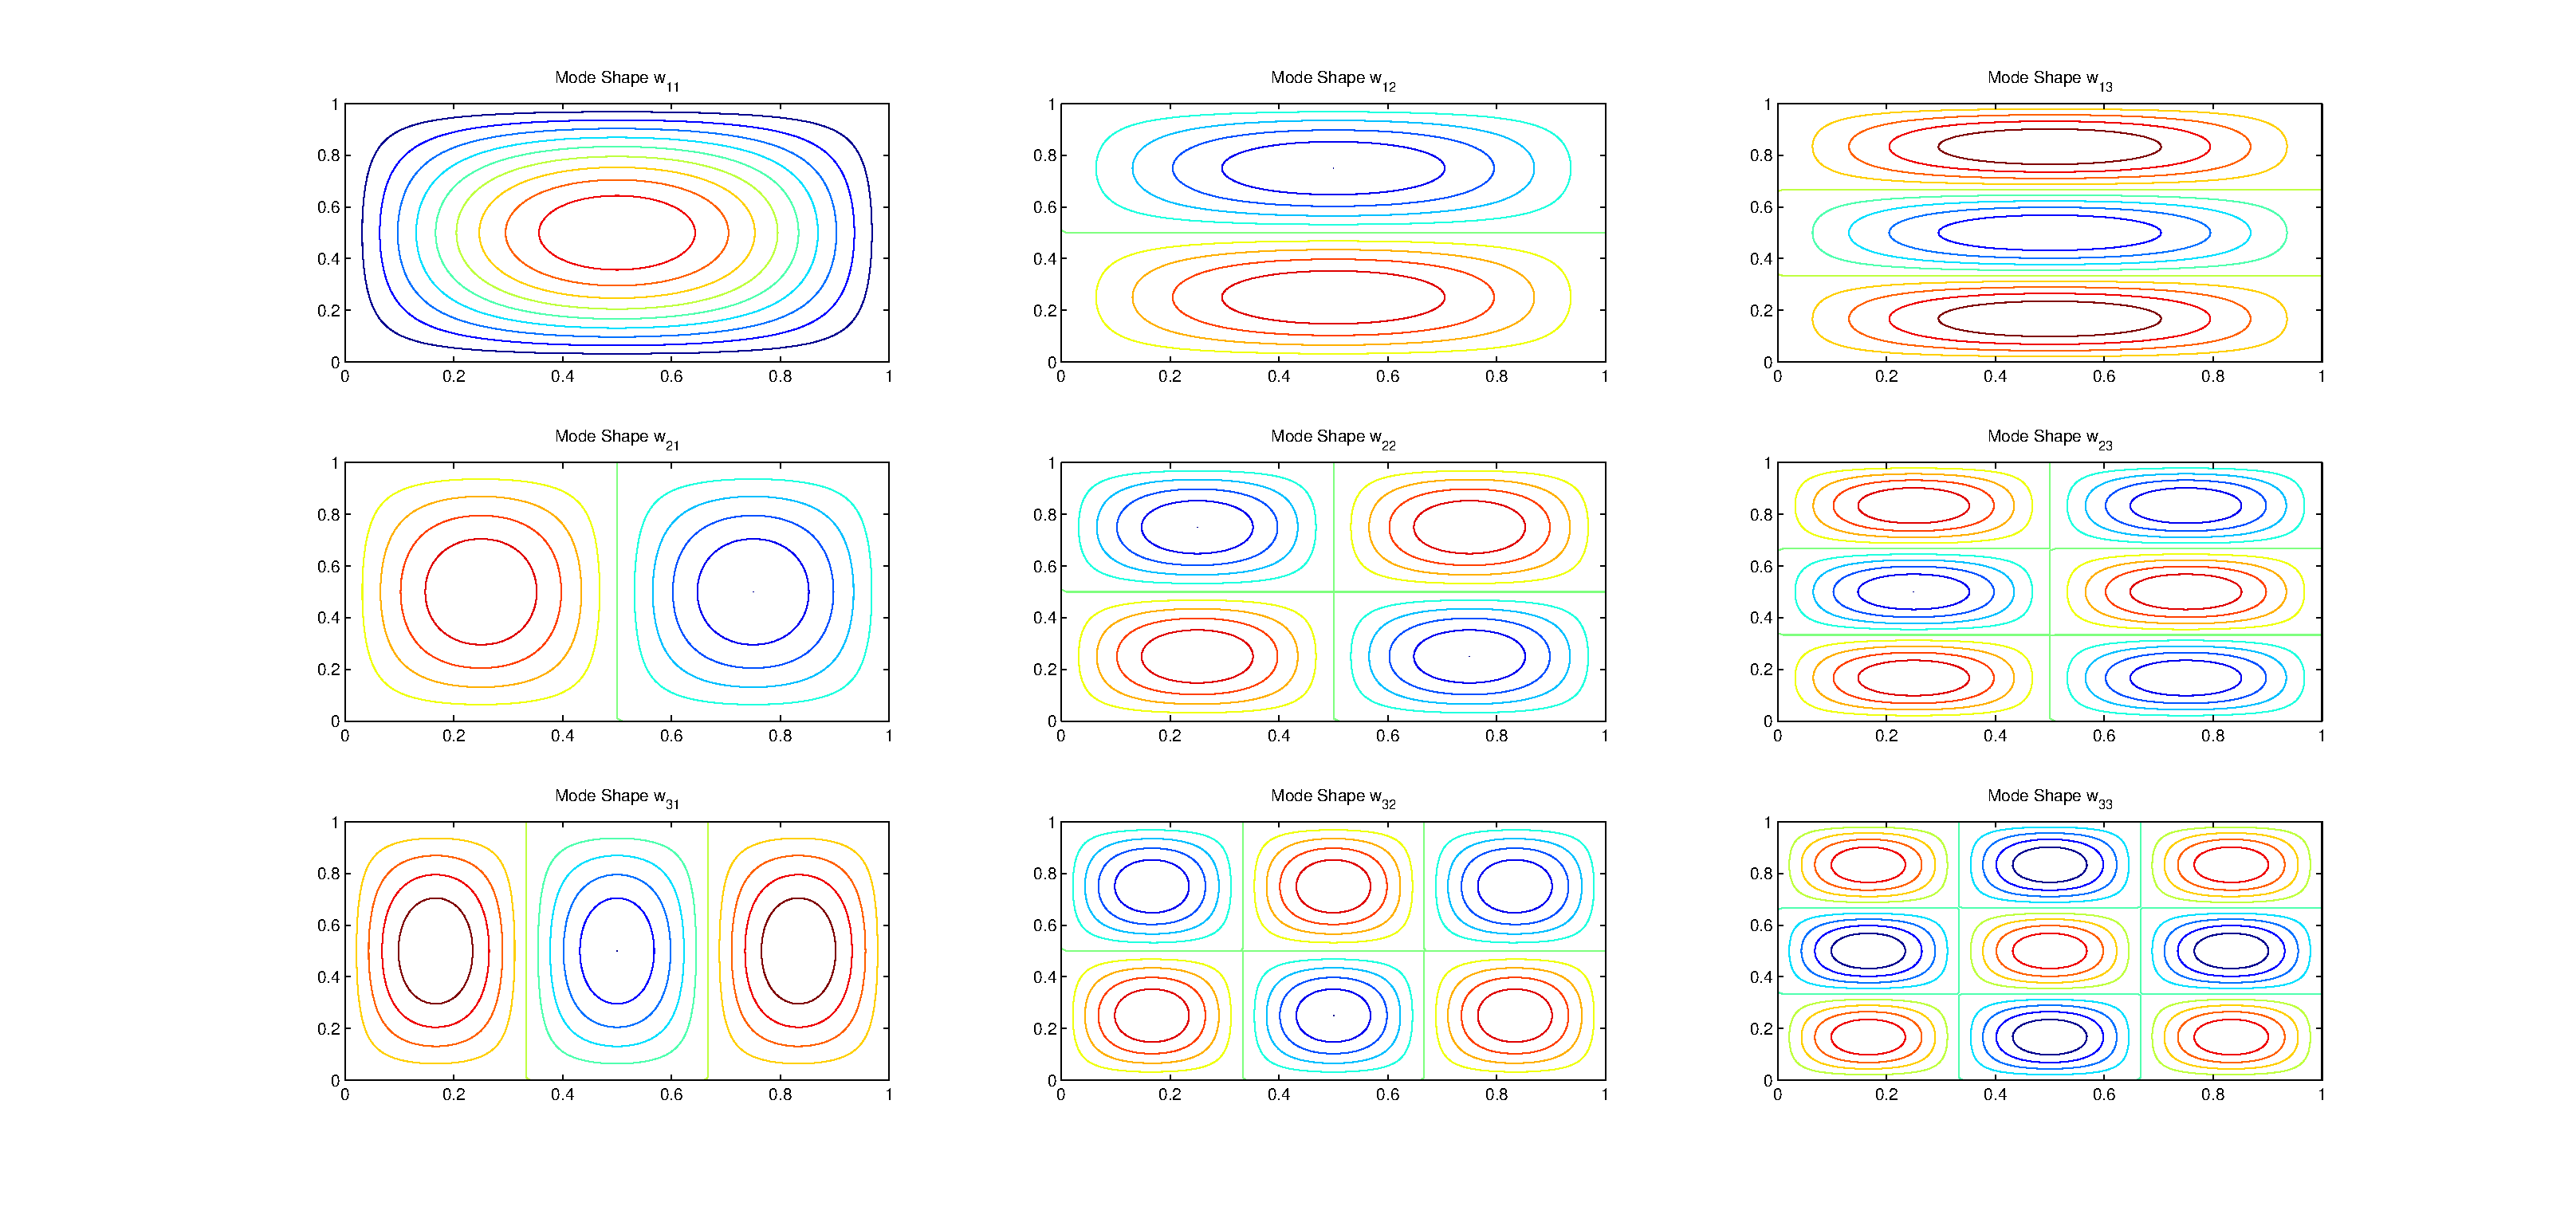
\includegraphics[width=\textwidth]{modes}
	\caption{Contour plots of selected mode shapes}
\end{figure}

\begin{figure}[h]
	\label{modes}
	\includegraphics[width=\textwidth]{modes_surf}
	\caption{Surface plots of selected mode shapes}
\end{figure}

% CONCLUSIONS
\section{Conclusions}

% BIBLIOGRAPHY
%\clearpage
%\addcontentsline{toc}{section}{Bibliography}
%\begin{thebibliography}{99}
%	\bibitem{bib:1} Nagle, Staff, Snider. \emph{Differential Equations and Boundary-Value Problems}.  Pearson Addison Wesley, fifth edition, 2008.
%\end{thebibliography}

% APPENDIX
\newpage
\section{Appendix}
\subsection{MATLAB script for plotting mode shapes}
\lstset{numbers=left, numberstyle=\tiny}
\lstinputlisting{mode_plotter.m}

\subsection{MATLAB script for plotting mode shapes}
\lstinputlisting{automate.m}

\subsection{Project responsibilities}
Daniel Geiyer had the following responsibilities:
\begin{enumerate}
	\item{Determine the appropriate FEA implementation of the project.}
	\item{Perform the FE analysis.}
\end{enumerate}
Sigitas Rimkus had the following responsibilities:
\begin{enumerate}
	\item{Research the mathematical basis of the problem.}
	\item{Find the required analytical solution(s) to the problem.}
	\end{enumerate}
The following responsibilities were shared by both team members:
\begin{enumerate}
	\item{Compare the solutions provided by both methods.}
	\item{Prepare the required project progress reports.}
	\item{Provide input for the desired content and layout of the final report and presentation.}
\end{enumerate}

\end{document}
